\chapter{Výsledková část}
Následující kapitola shrnuje získané výsledky pomocí CFD simulace popsané v předcházejících odstavcích. 

Na obr. \ref{fig:vecfield} je znázorněno vektorové pole rychlosti kapaliny v řezu nádobou a čase \SI{6}{\second}, což již lze považovat za poměrně ustálený stav. Z obrázku je dobře patrný vznikl sekundárních cirkulačních smyček v prostoru pod míchadlem. Tento jev byl experimentálně pozorován řadou autorů (např. \citet{hos10}) při zvolené světlé výšce míchadla od $C=T/2$ do $C=T/6$.  

\begin{figure}[h!]
\begin{center}
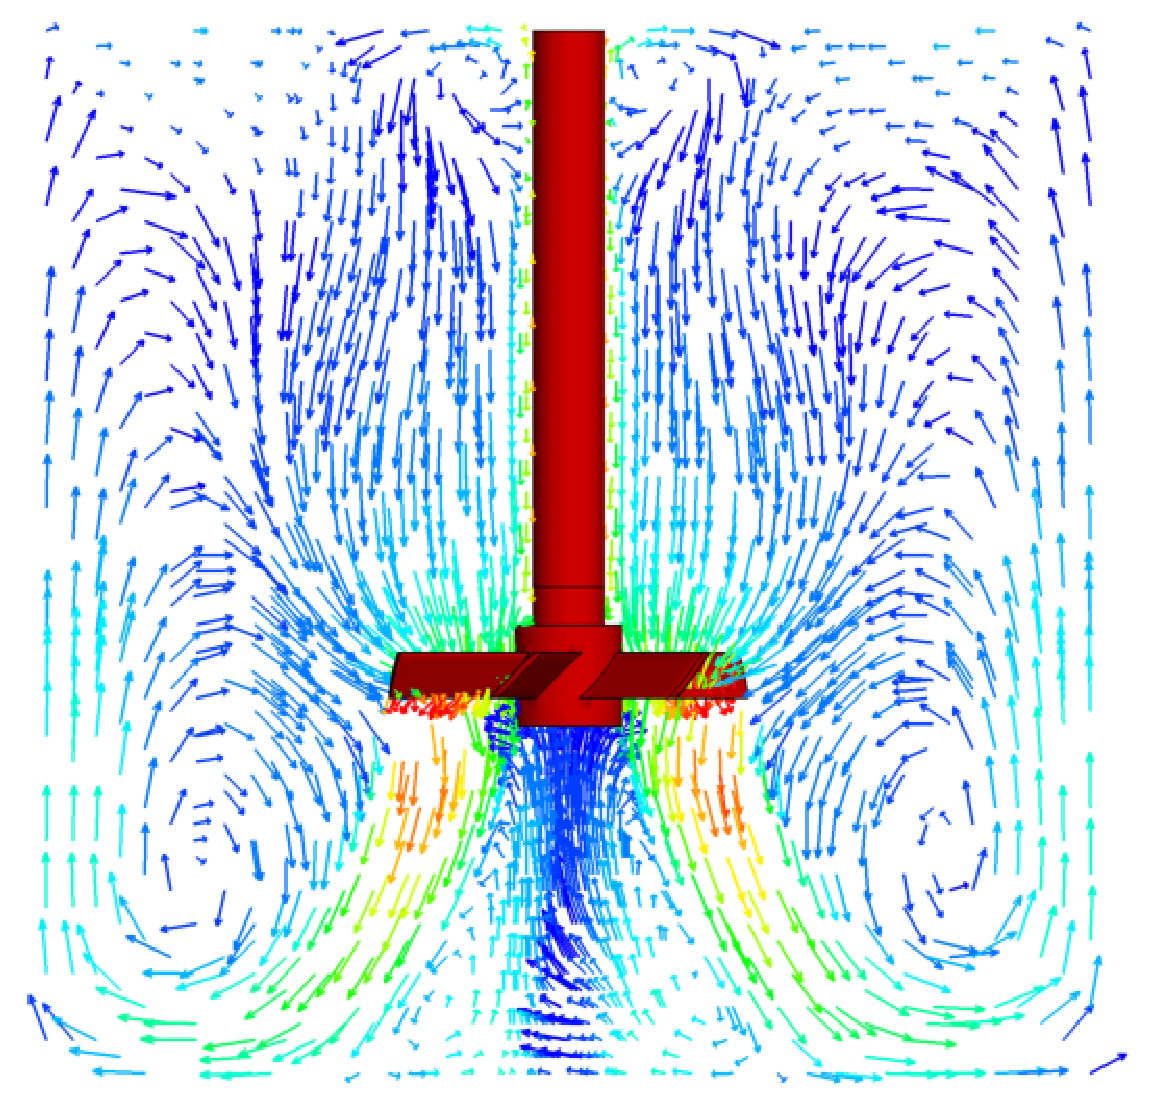
\includegraphics[scale=0.5]{images/vecfield.eps}
\caption{Vektorové pole rychlosti}
\label{fig:vecfield}
\end{center}
\end{figure} 

\vspace{-9mm}

Obr. \ref{fig:count2} zobrazuje kontury objemového zlomku pevné fáze v řezu míchací nádobou pro vybrané korelace odporového koeficientu. Tyto údaje byly získány v času simulace \SI{2}{\second}. Z obrázků je dobře patrné, že přímo pod míchadlem je největší koncentrace pevné fáze vlivem sekundárních cirkulačních smyček. Korelace odporového koeficientu podle \hyperlink{hyp:cds}{Brucata} v tomto případě předpovídá významně vyšší rozložení kuliček z PVC pod míchadlem než zbývající modely.

\newpage

\begin{figure}[h!]
  \begin{center}
  \subfloat[\hyperlink{hyp:schlneu}{Schiller-Naumann}]{\label{fig:neu2}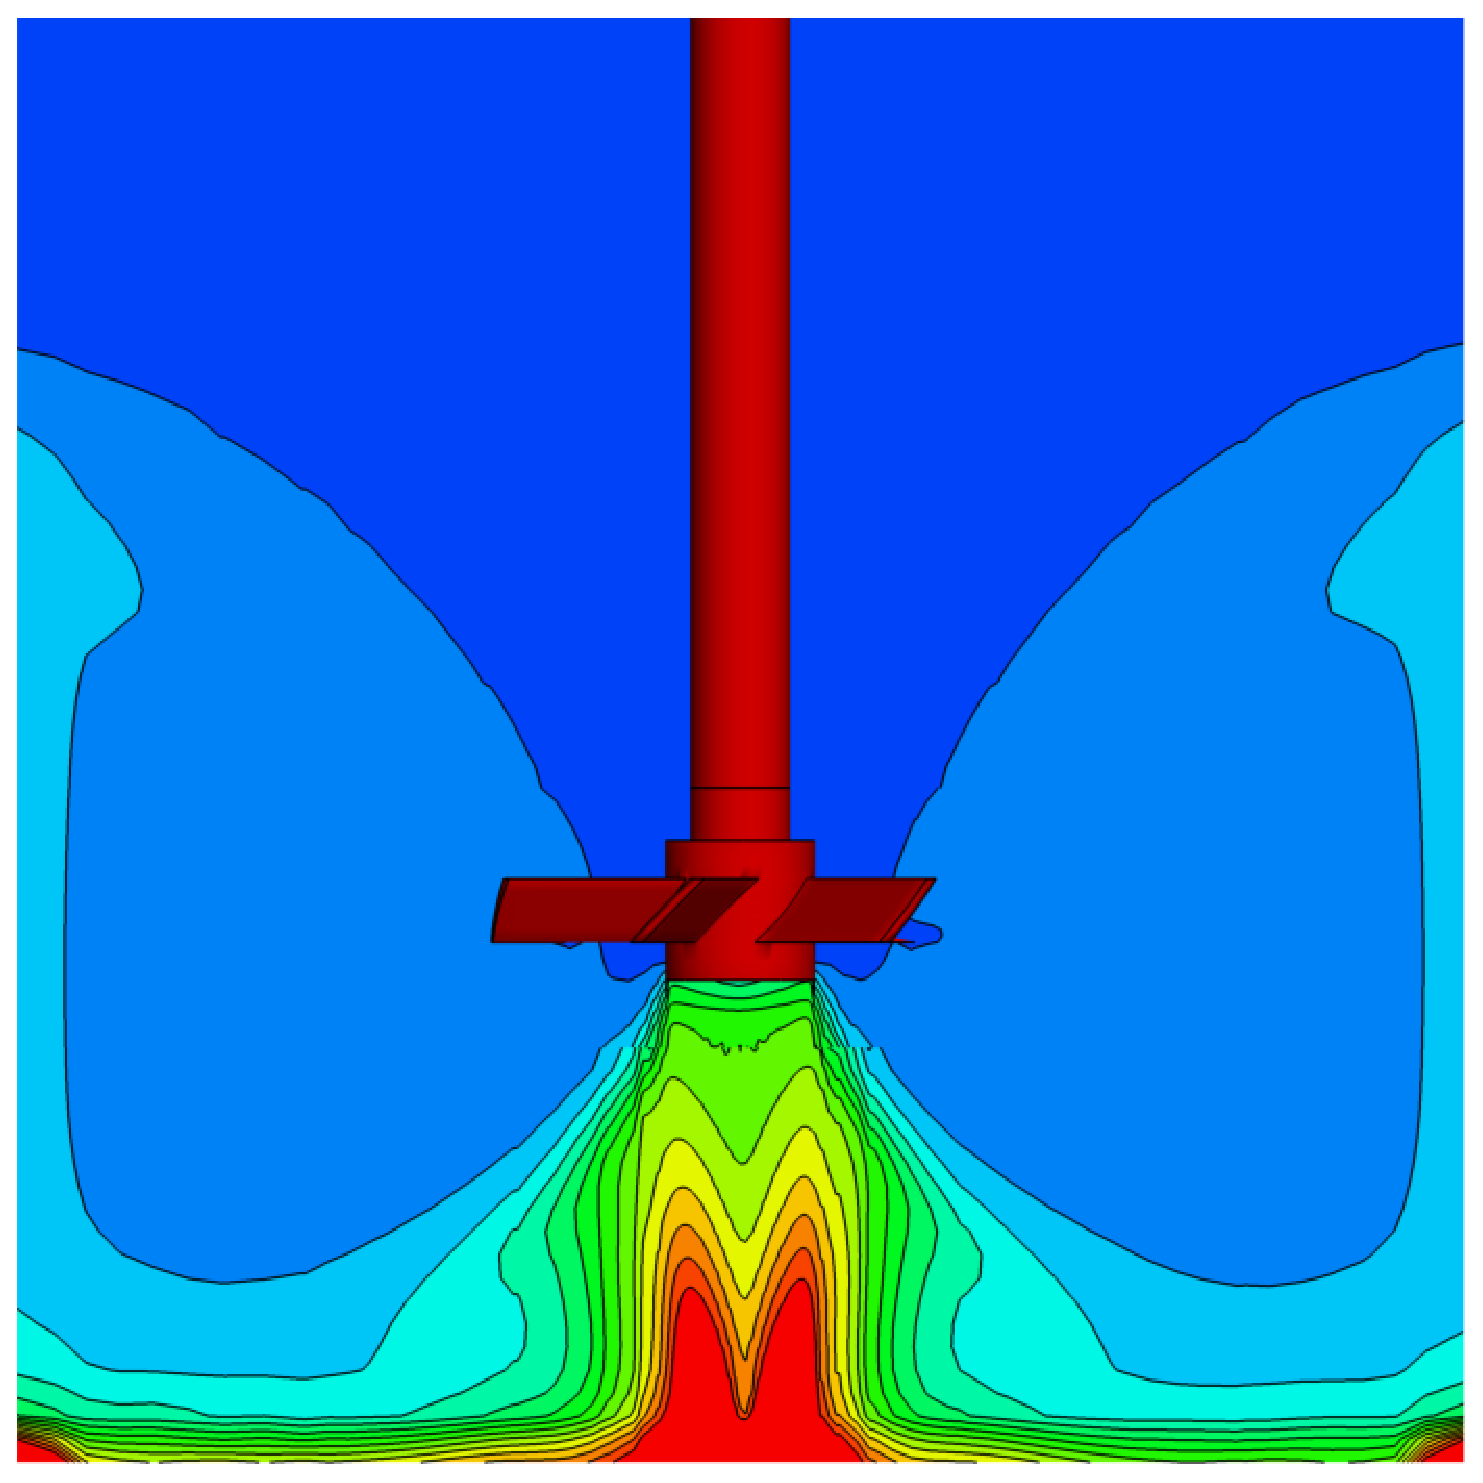
\includegraphics[scale=0.3]{images/volSch-2.eps}}  
  \qquad             
  \subfloat[\hyperlink{hyp:cds}{Pinelli}]{\label{fig:pin2}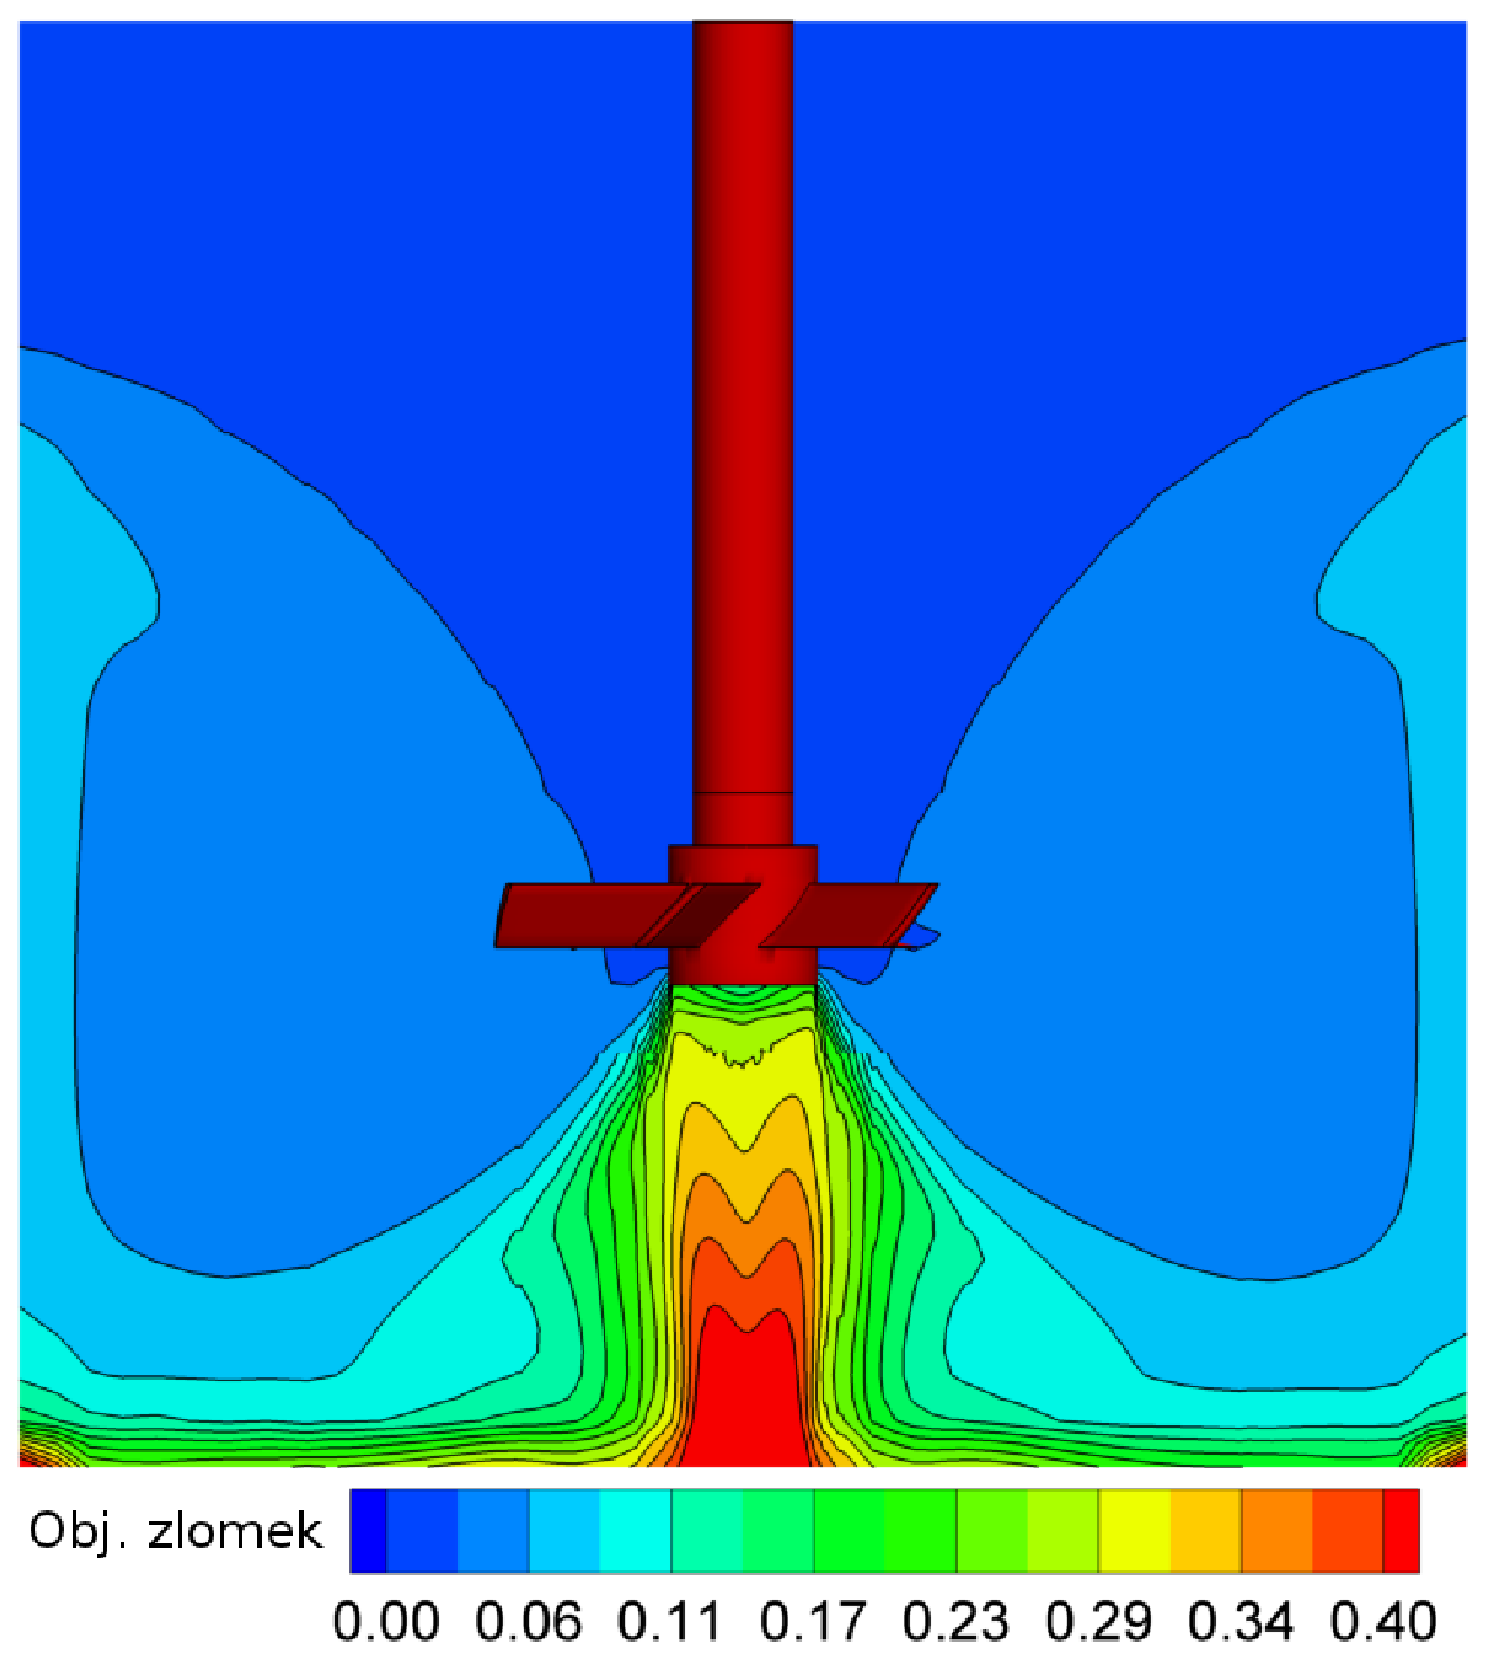
\includegraphics[scale=0.3]{images/volPin-2.eps}}
  \\
  \subfloat[\hyperlink{hyp:cds}{Brucato}]{\label{fig:bru2}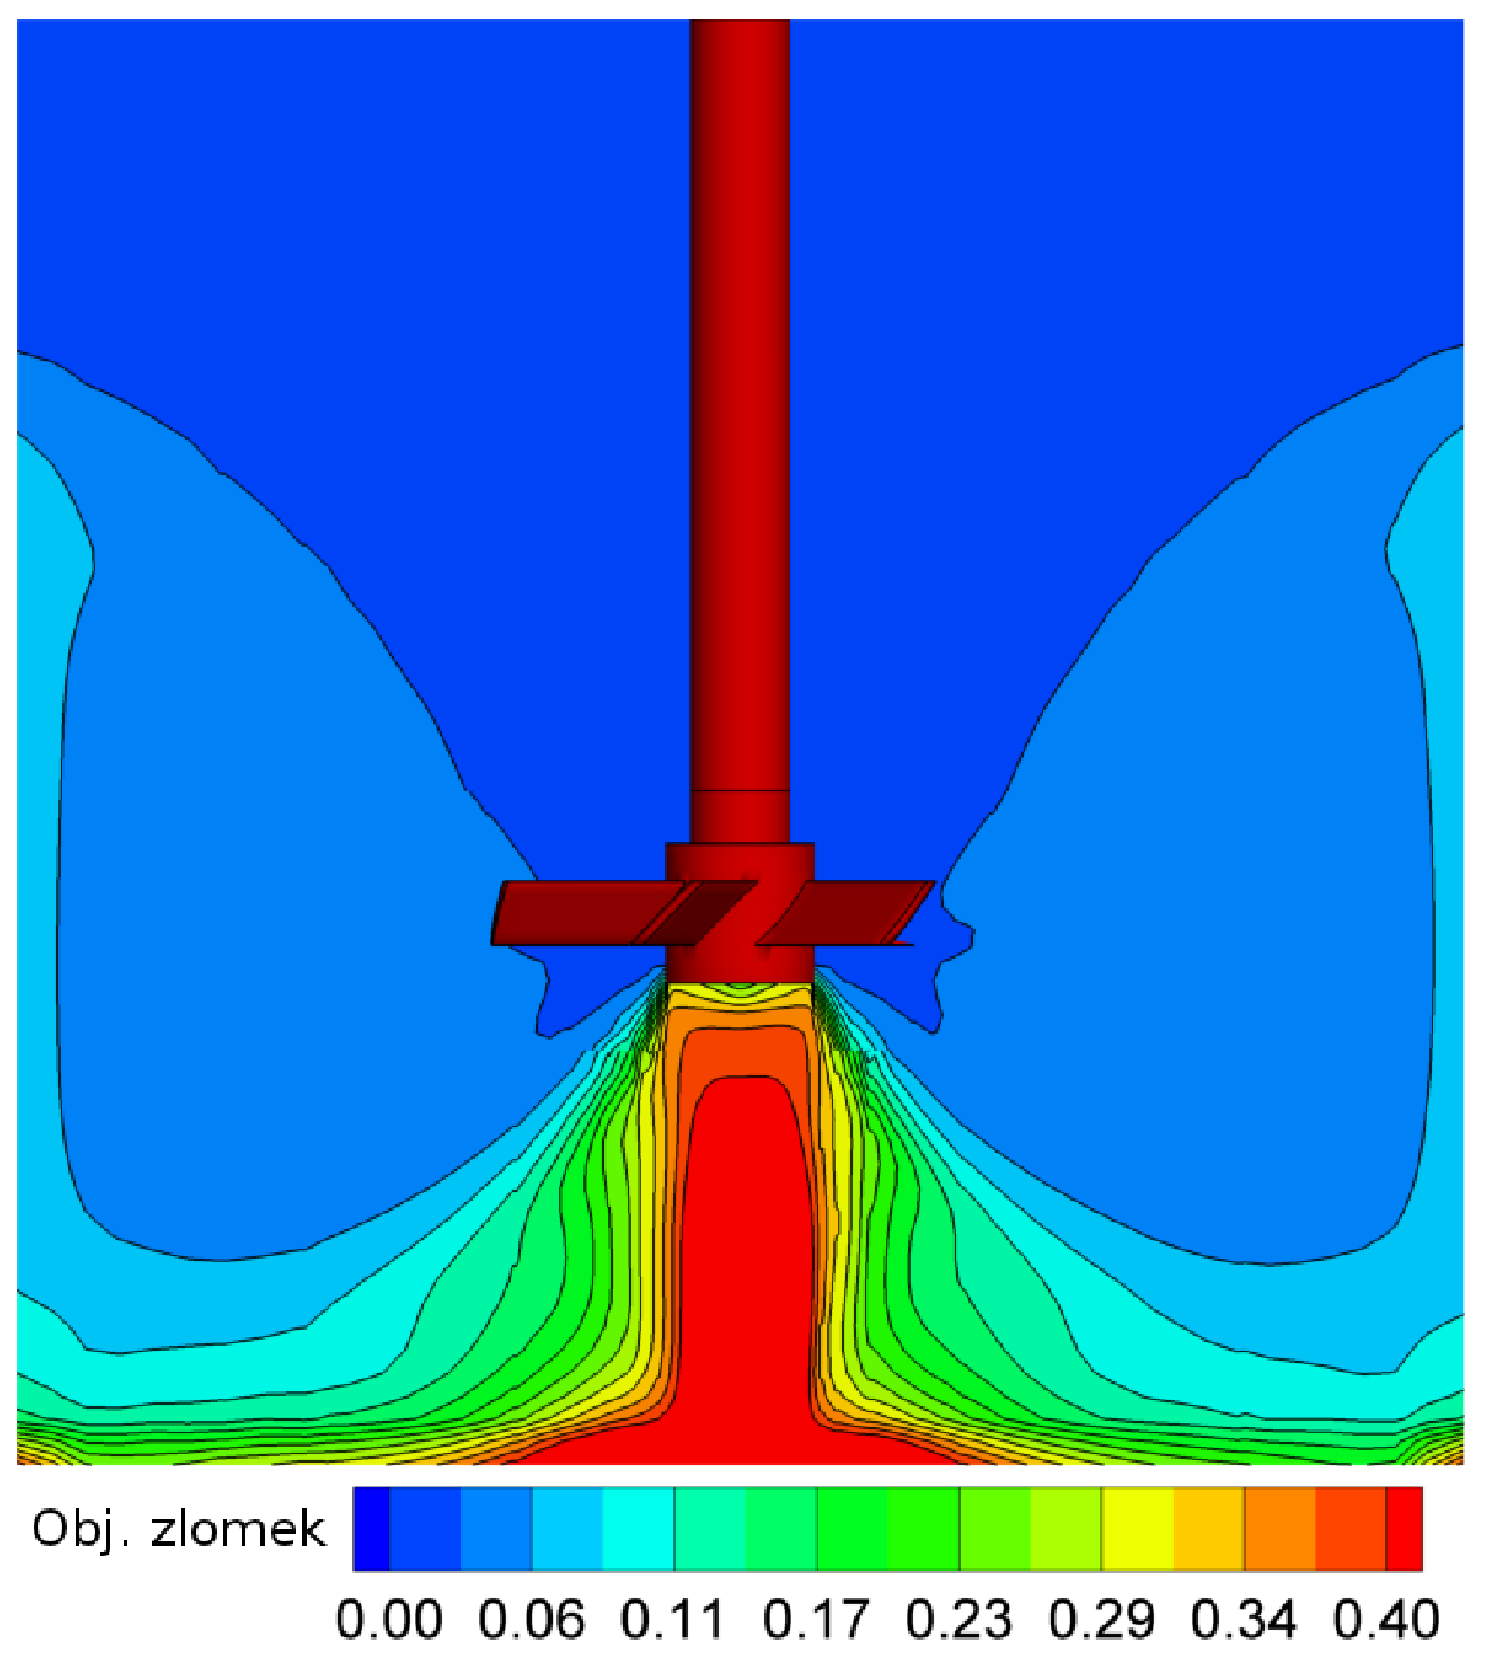
\includegraphics[scale=0.3]{images/volBru-2.eps}}
  \qquad
  \subfloat[\hyperlink{hyp:cds}{Khopkar}]{\label{fig:kho2}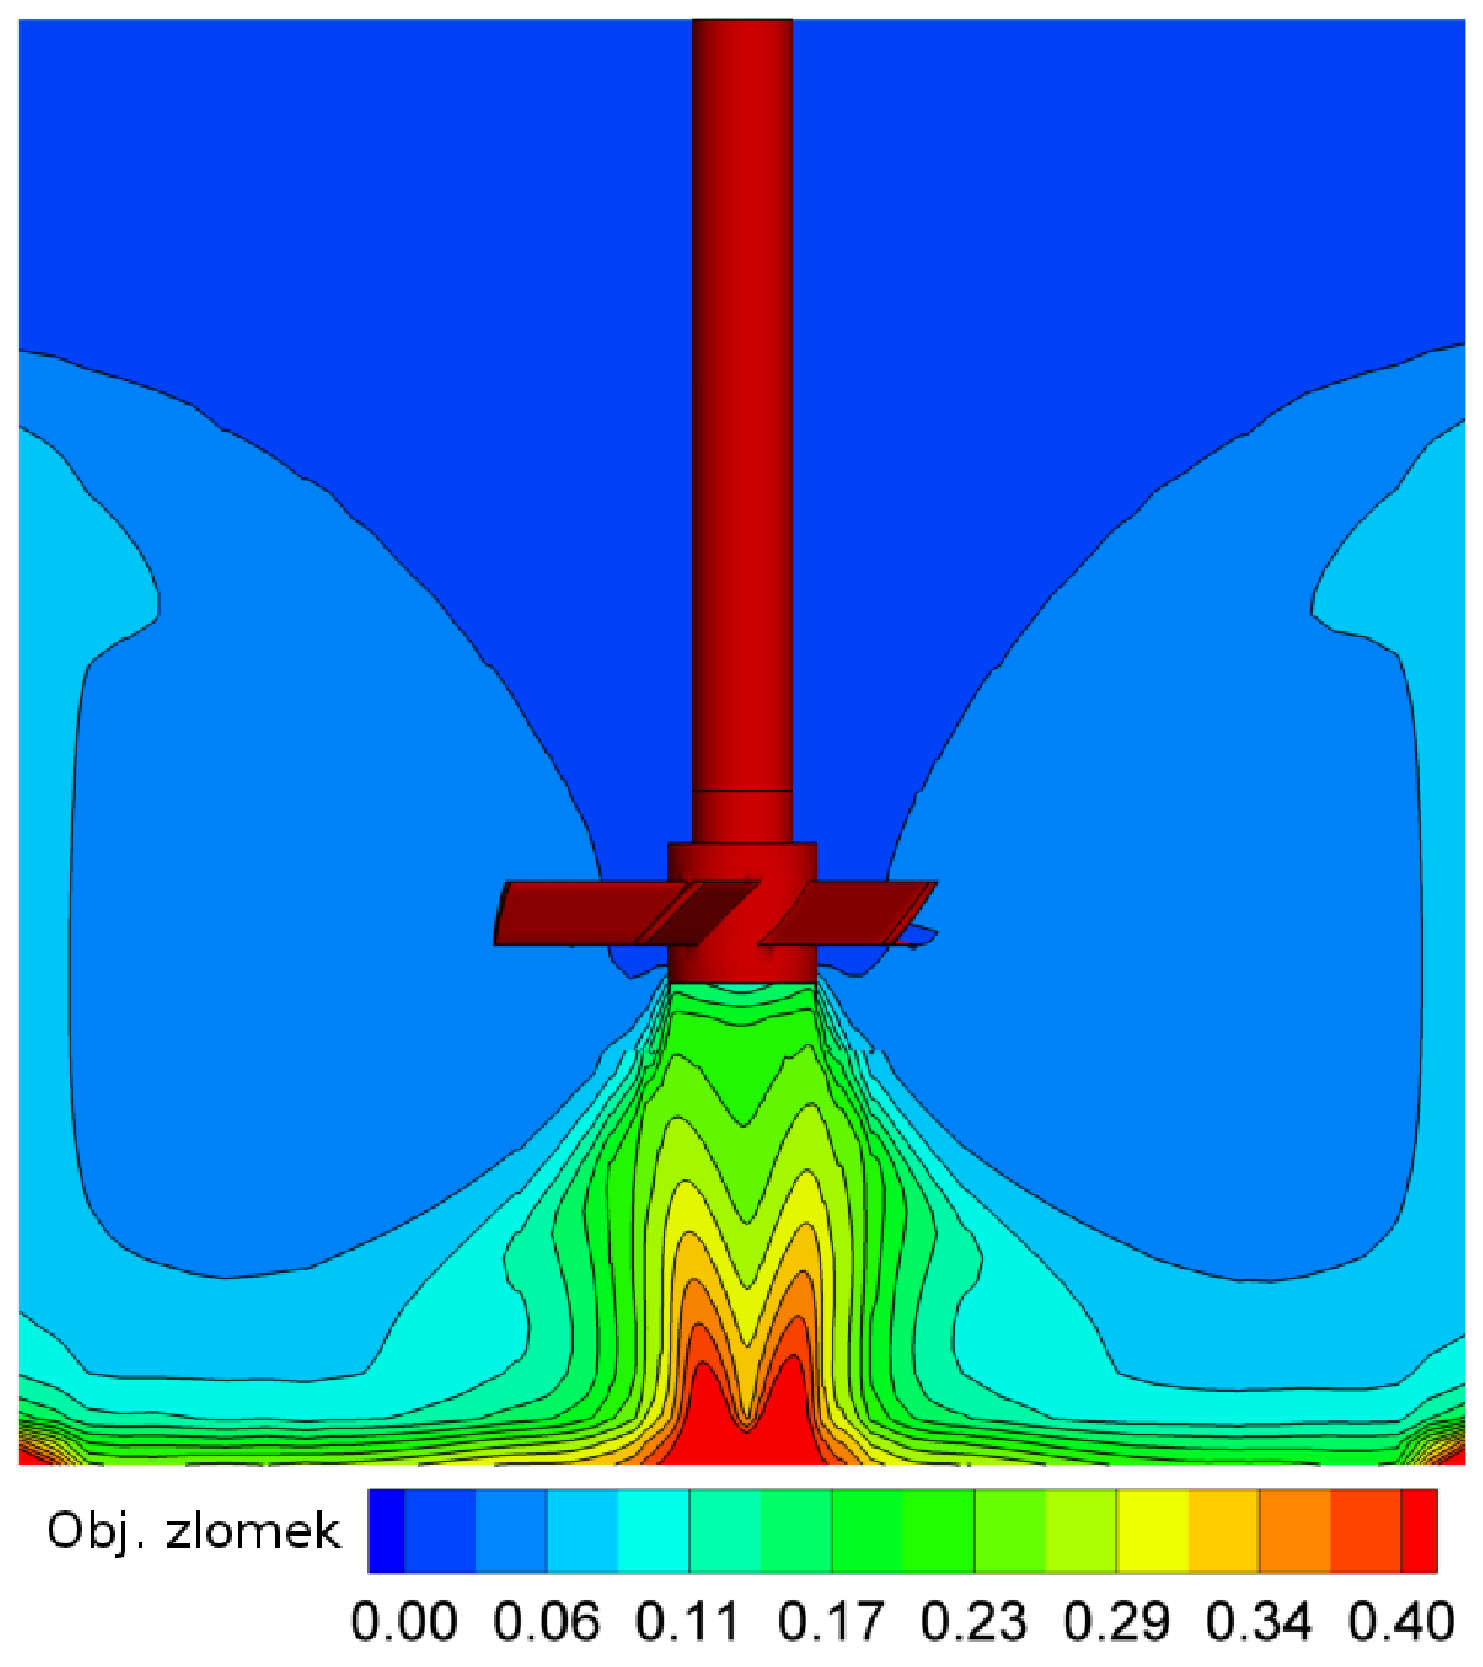
\includegraphics[scale=0.3]{images/volKho-2.eps}}
  \caption{Objemový zlomek fáze v čase \SI{2}{\second}}
  \label{fig:count2}
  \end{center}
\end{figure}

\vspace{-9mm}

Následují opět obrázky zachycují objemový zlomek pevné fáze v řezu nádobou, avšak v tomto případě pro čas \SI{6}{\second}. Pevná fáze je již poměrně rozptýlena, ale stále se pod míchadlem nacházejí oblasti se zvýšenými koncentracemi.

\newpage

\begin{figure}[h!]
  \begin{center}
  \subfloat[\hyperlink{hyp:schlneu}{Schiller-Naumann}]{\label{fig:neu6}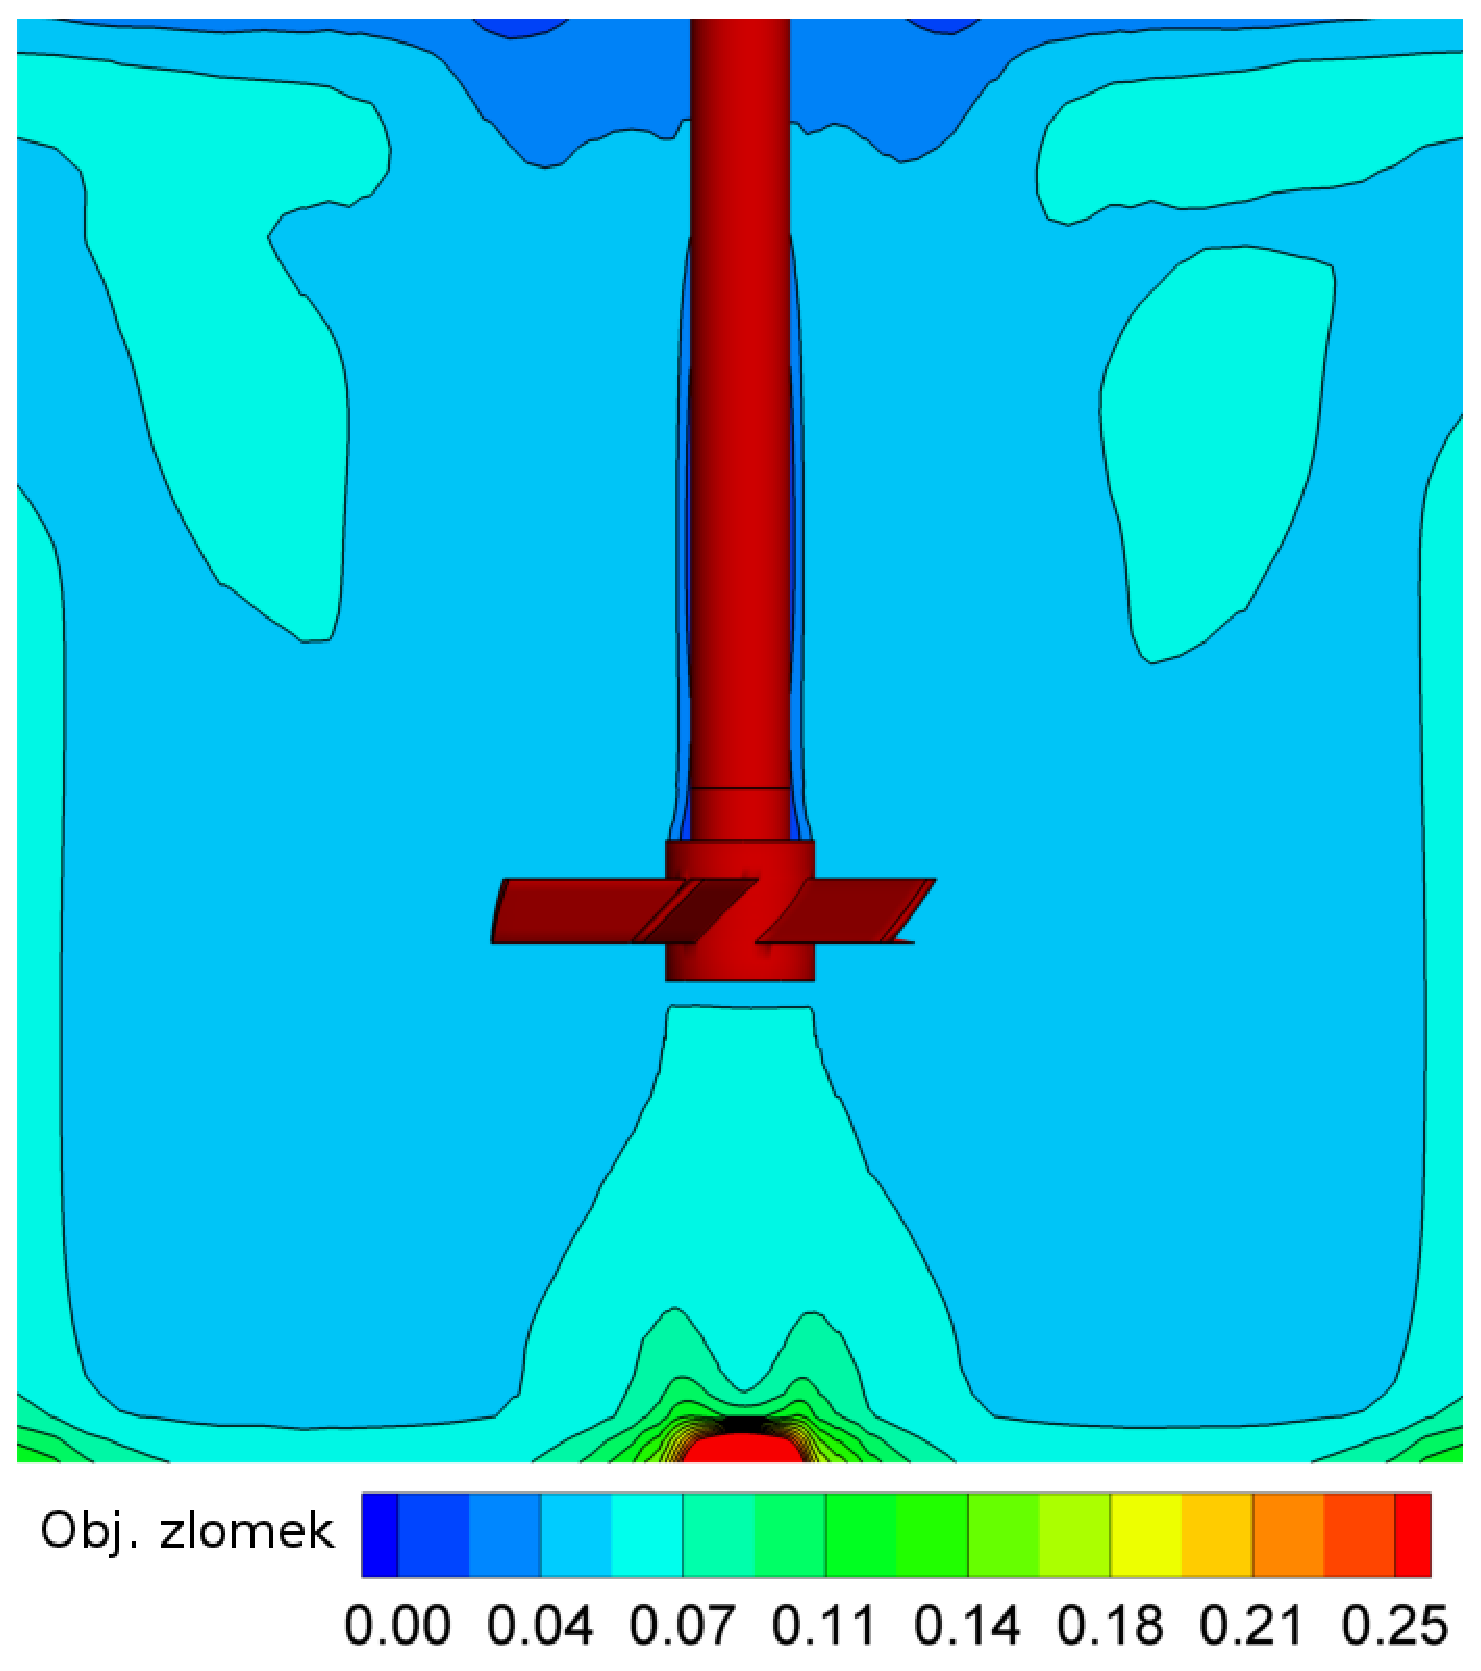
\includegraphics[scale=0.3]{images/volSch-6.eps}}  
  \qquad             
  \subfloat[\hyperlink{hyp:cds}{Pinelli}]{\label{fig:pin6}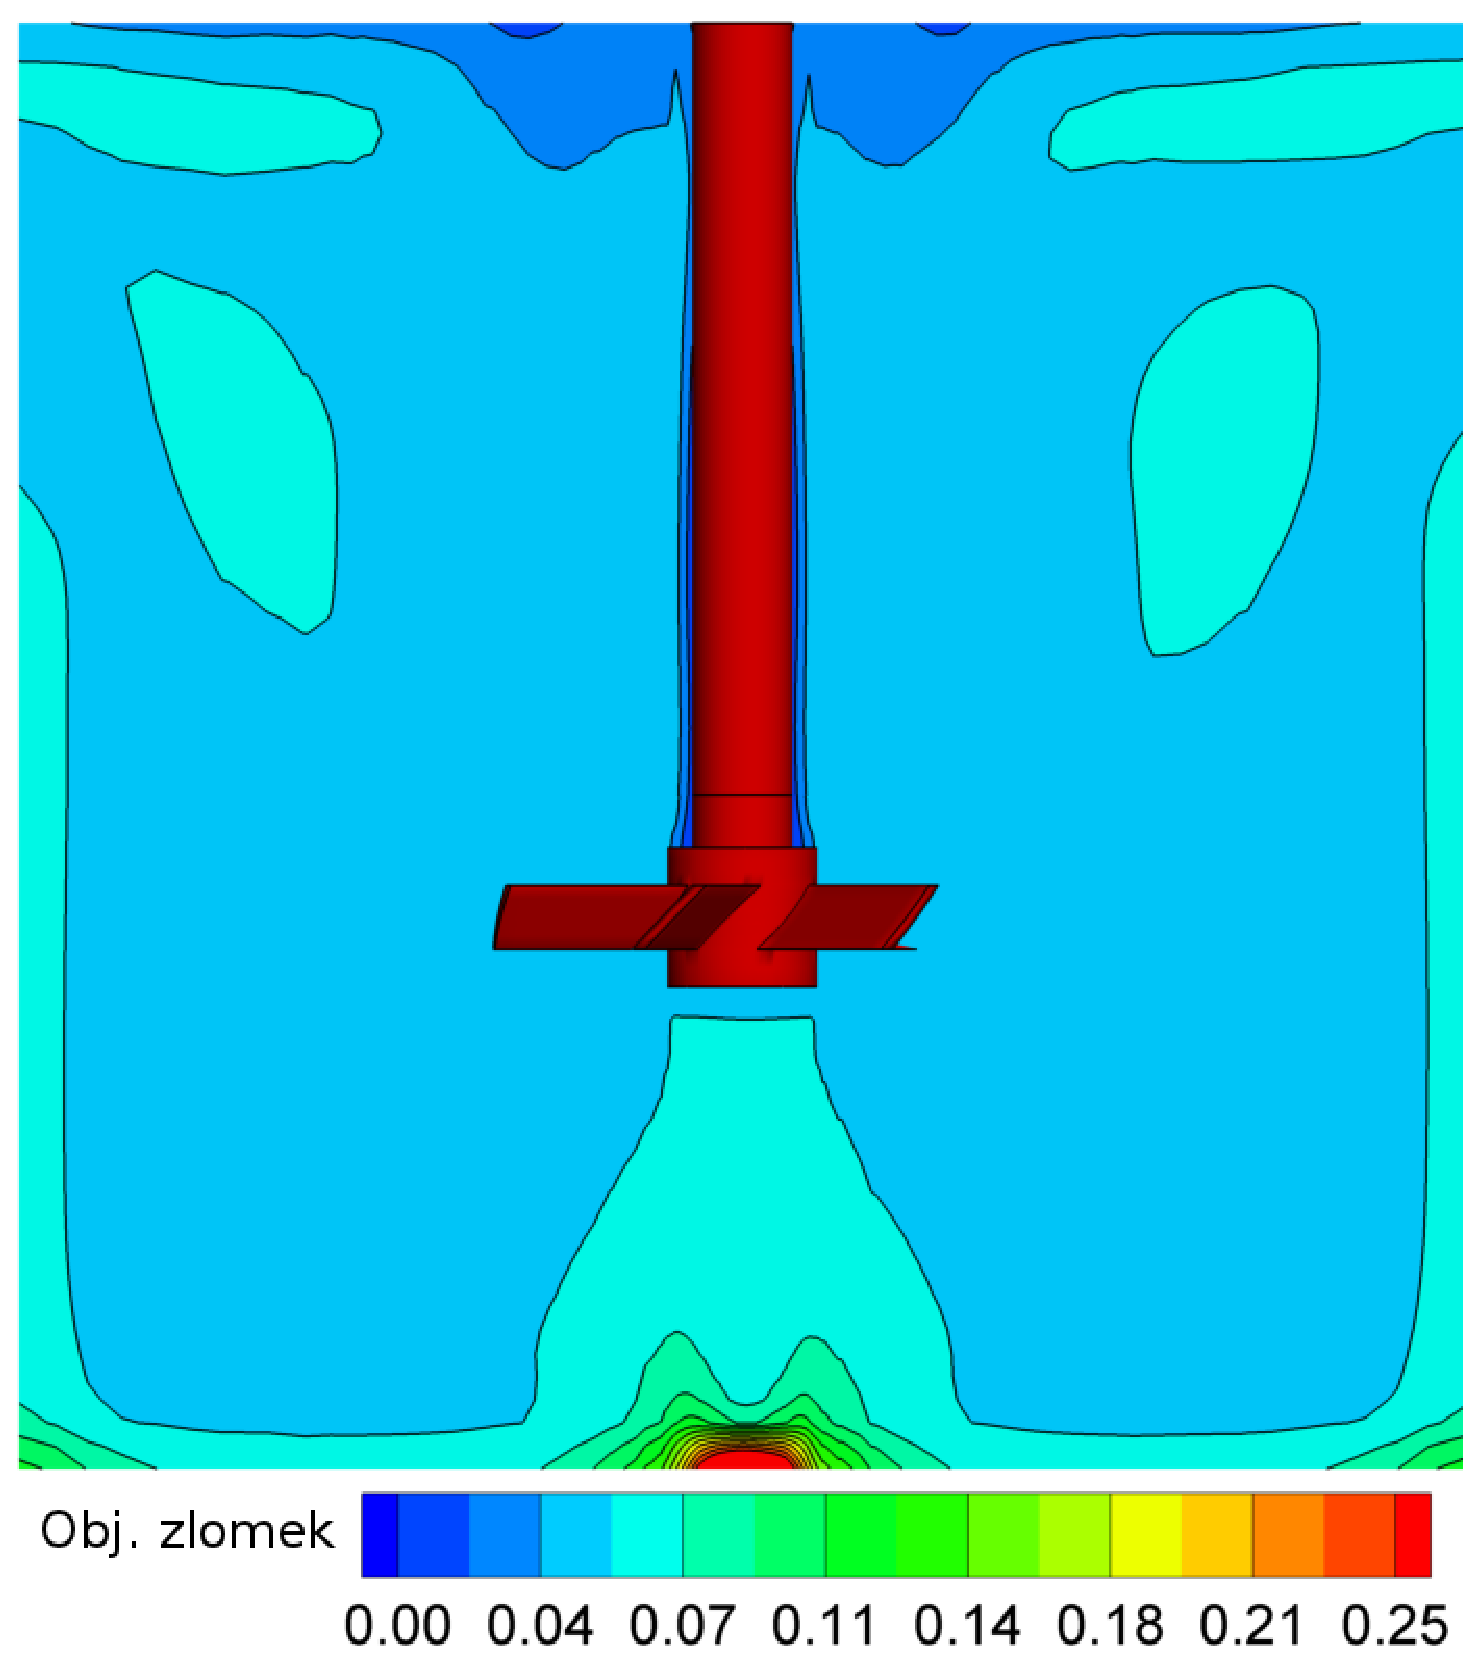
\includegraphics[scale=0.3]{images/volPin-6.eps}}
  \\
  \subfloat[\hyperlink{hyp:cds}{Brucato}]{\label{fig:bru6}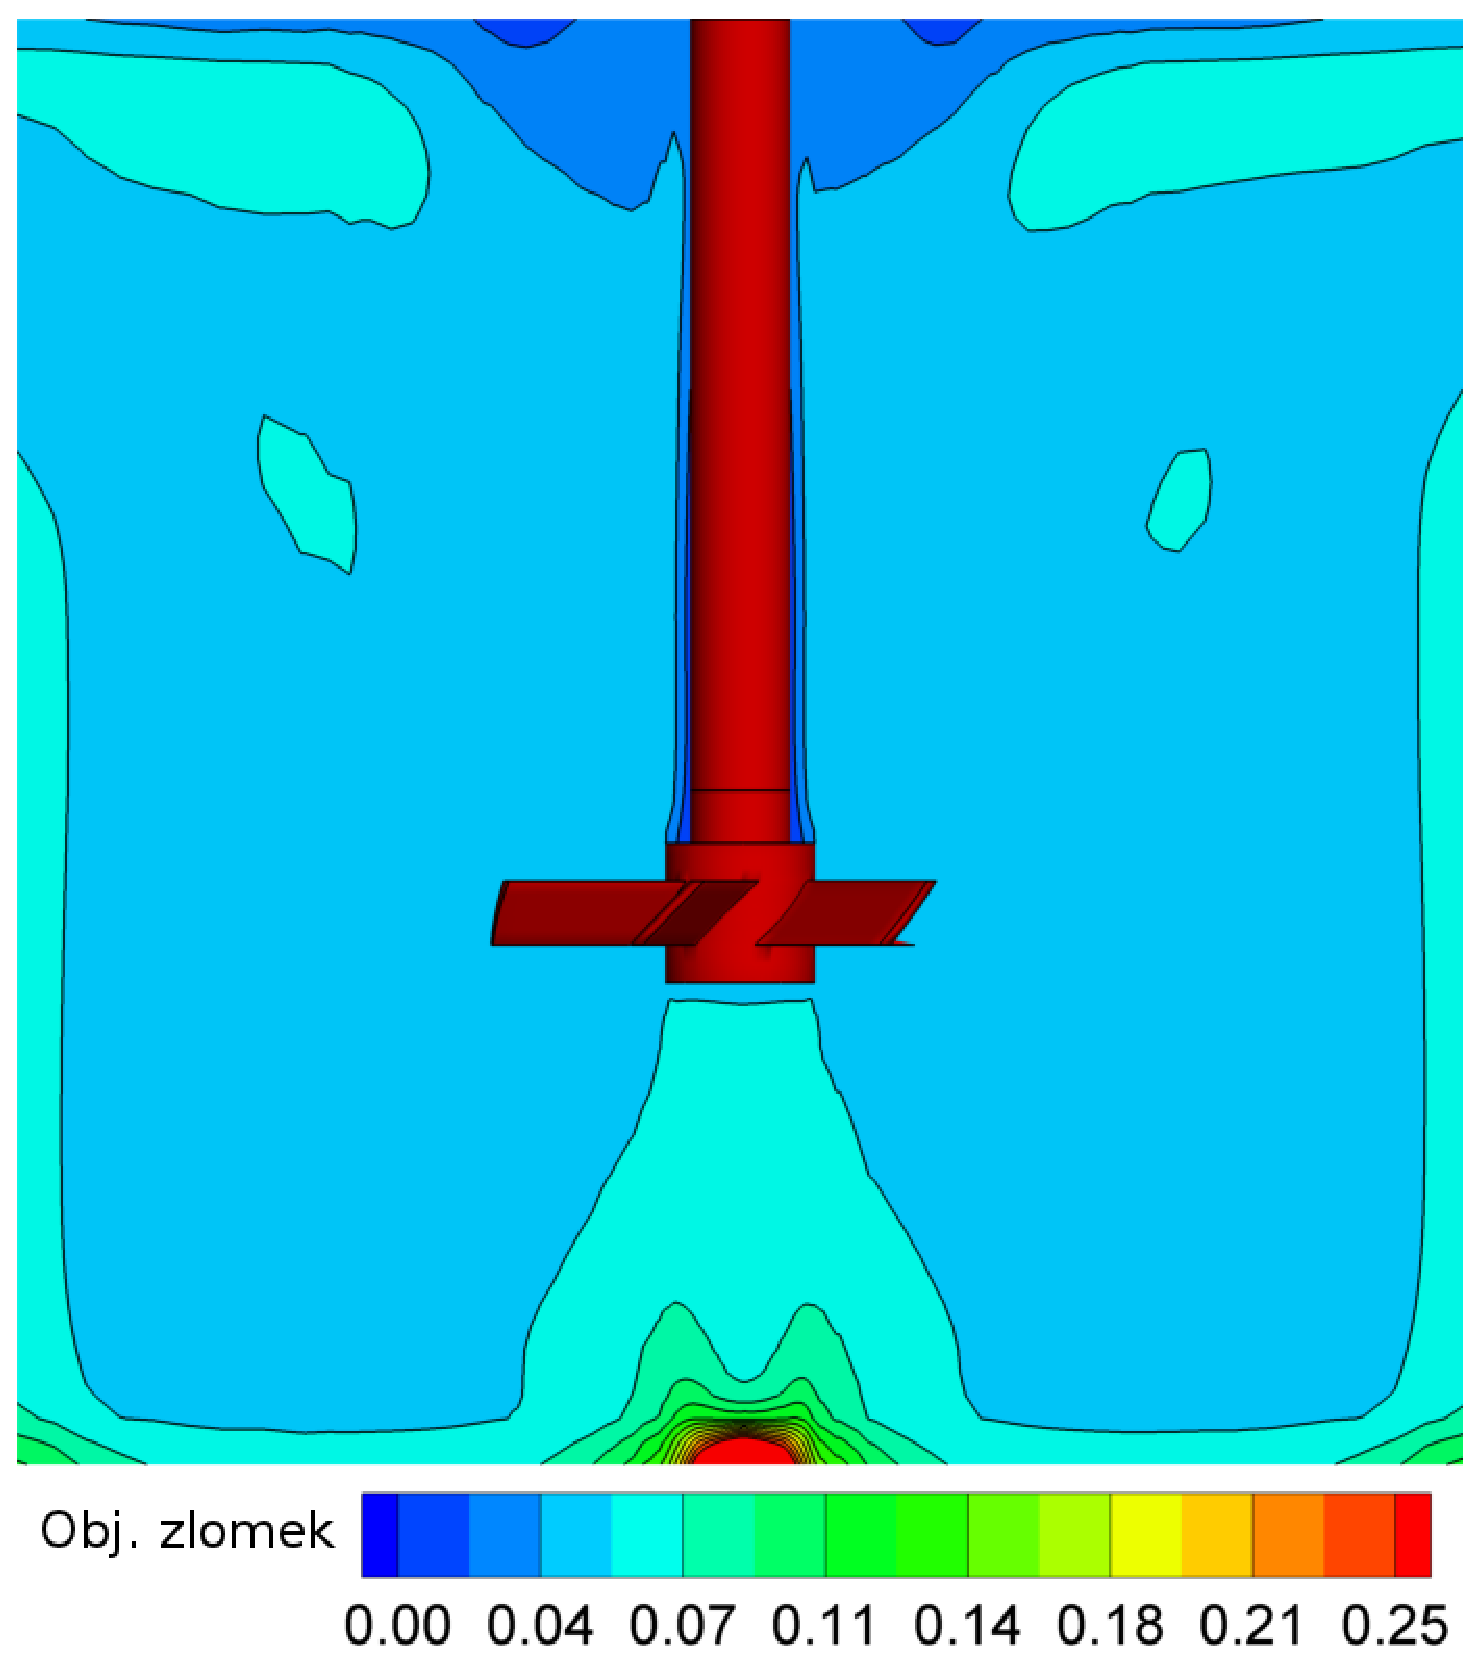
\includegraphics[scale=0.3]{images/volBru-6.eps}}
  \qquad
  \subfloat[\hyperlink{hyp:cds}{Khopkar}]{\label{fig:kho6}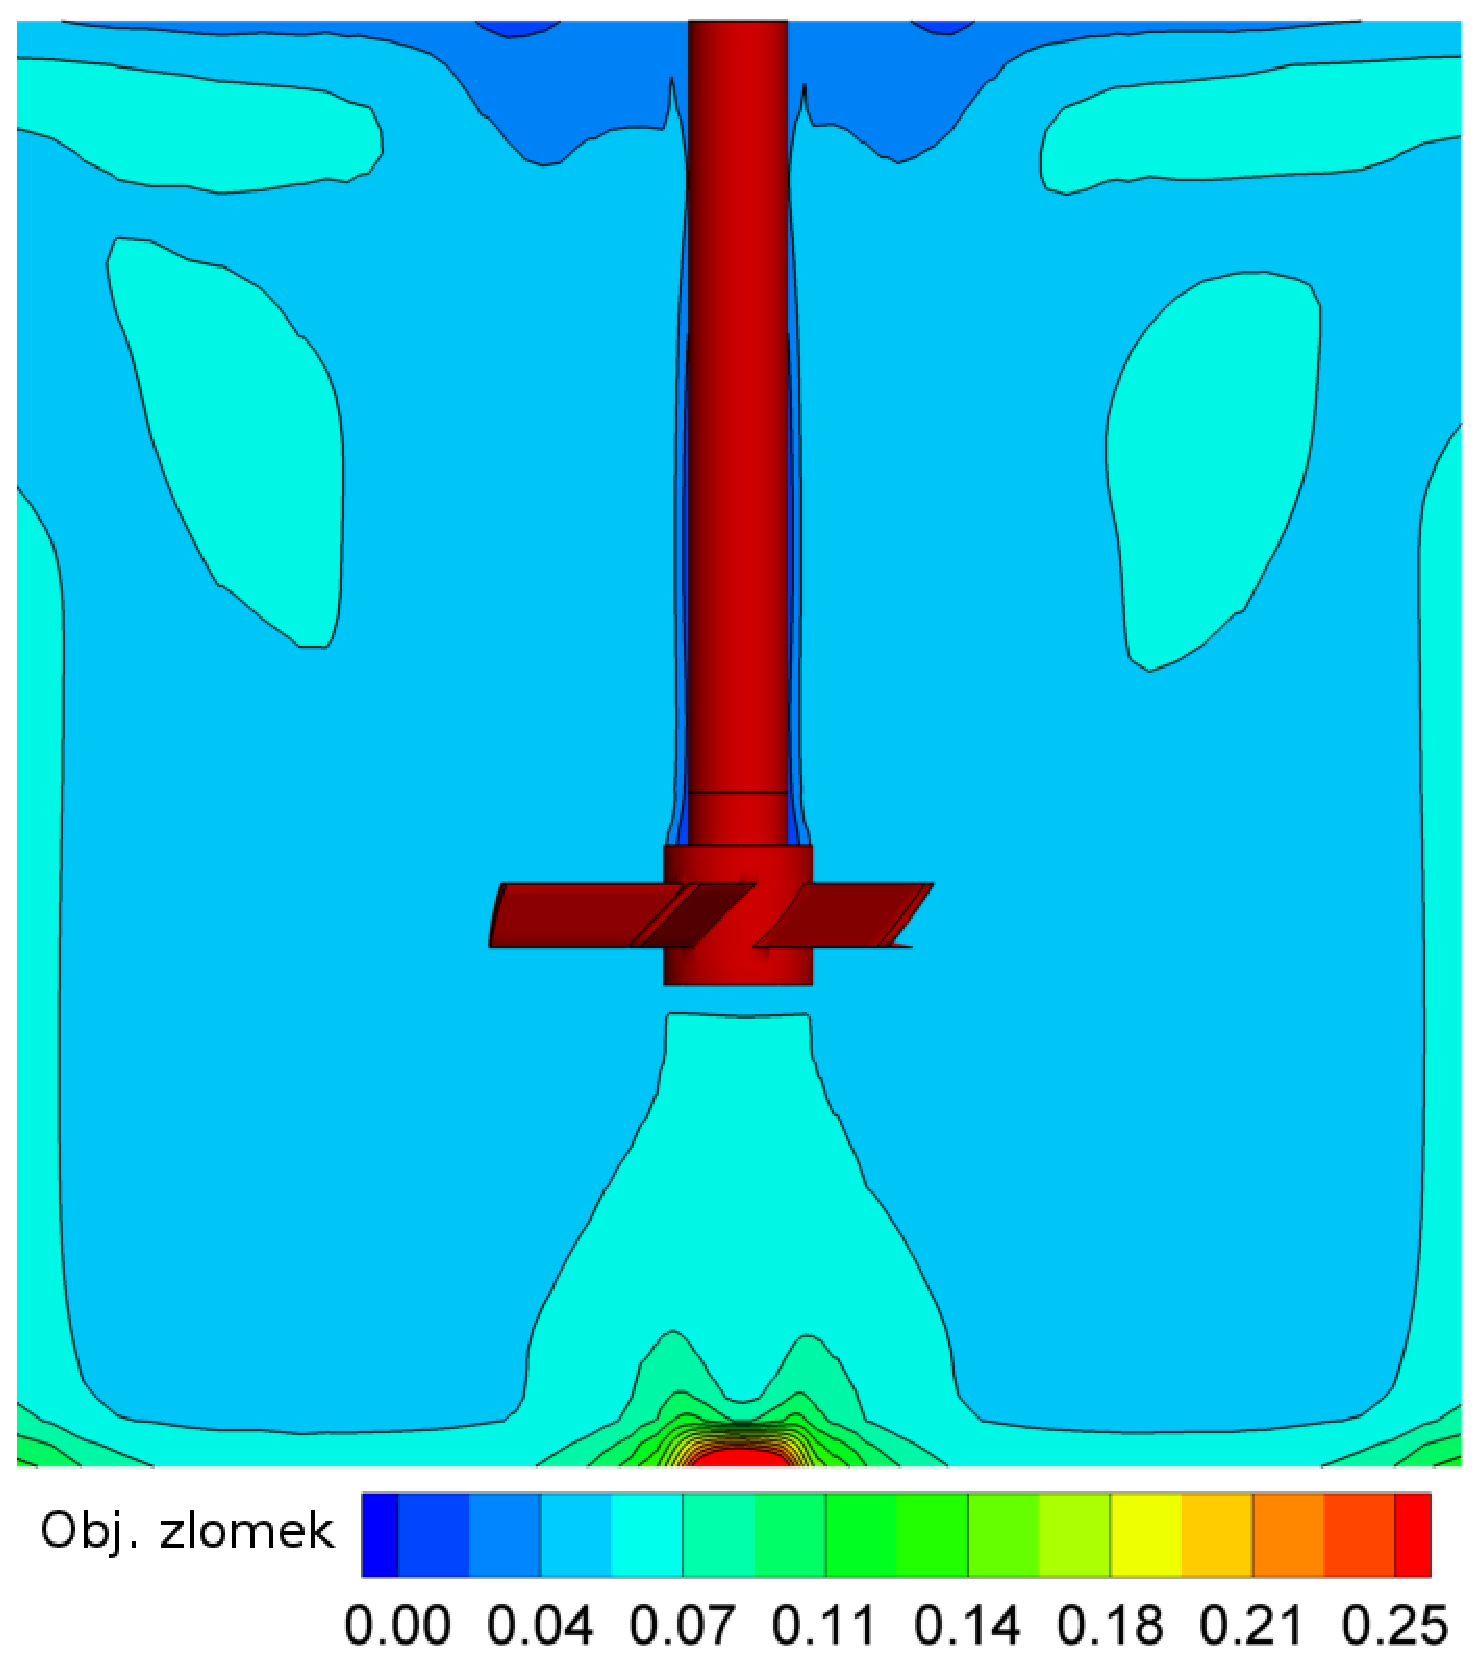
\includegraphics[scale=0.3]{images/volKho-6.eps}}
  \caption{Objemový zlomek pevné fáze v čase \SI{6}{\second}}
  \label{fig:count6}
  \end{center}
\end{figure}

\vspace{-9mm}

Dále jsou zde uvedeny grafické závislosti vzdálenosti ode dna nádoby na objemovém zlomku pevné fáze. Údaje pro tyto grafy byly získány stanovením objemového zlomku pevné fáze podél úsečky rovnoběžné s osou míchadla ve vzdálenosti \SI{11}{\centi\metre}.

Z obr. \ref{fig:vol2} je dobře patrné, že s rostoucí vzdáleností ode dna se koncentrace pevné fáze postupně snižuje. Avšak grafická závislosti nemá monotonní průběh, přičemž dochází k tvorbě esovitého koncentračního profilu. Model koeficientu odporu navržený \hyperlink{hyp:cds}{Brucatem} předpovídá nižší koncentraci pevné fáze ve vyšší vzdálenosti ode dna než zbýlé tři modely.     

\newpage

\begin{figure}[h!]
\begin{center}
\includegraphics[scale=0.47]{images/Vol-2.eps}
\caption{Průběh objemového zlomku pevné fáze v čase \SI{2}{\second}}
\label{fig:vol2}
\end{center}
\end{figure} 

\vspace{-9mm}

\noindent V čase \SI{6}{\second} kuličky z PVC již dosáhnout značného vznosu a opět si lze povšimnout z obr. \ref{fig:vol6}, že \hyperlink{hyp:cds}{Brucatova} korelace se stále nejvýznamněji odlišuje.  

\begin{figure}[h!]
\begin{center}
\includegraphics[scale=0.47]{images/Vol-6.eps}
\caption{Průběh objemového zlomku pevné fáze v čase \SI{6}{\second}}
\label{fig:vol6}
\end{center}
\end{figure} 

\vspace{-12mm}

\newpage

Na obr. \ref{fig:cd2} a \ref{fig:cd6} jsou vyneseny závislosti vzdálenosti ode dna nádoby na hodnotě odporového koeficienty v čase \SI{2}{\second} resp. \SI{6}{\second}. V obou případech mají hodnoty koeficientu odporu podobný průběh pro různé korelace, nicméně z obr. \ref{fig:cd2} je zřejmé, že blízko dna nádoby, kde objemový zlomek pevné fáze ve větší než   

\begin{figure}[h!]
\begin{center}
\includegraphics[scale=0.47]{images/CD-2.eps}
\caption{Průběh hodnoty odporového koeficientu v čase \SI{2}{\second}}
\label{fig:cd2}
\end{center}
\end{figure} 

\vspace{-12mm}

\begin{figure}[h!]
\begin{center}
\includegraphics[scale=0.47]{images/CD-6.eps}
\caption{Průběh hodnoty odporového koeficientu v čase \SI{6}{\second}}
\label{fig:cd6}
\end{center}
\end{figure} 

\vspace{-12mm}